%%%% 参考了https://www.wondercv.com/的模板

\documentclass[11pt]{article}

% disable indent globally
\setlength{\parindent}{0pt}
% some general improvements, defines the XeTeX logo
\usepackage{xltxtra}
% use hyperlink for email and url
\usepackage{hyperref}
\hypersetup{hidelinks}
\usepackage{url}
\urlstyle{tt}

\usepackage{xcolor}
%%%% 统一一种颜色,偏蓝色,用于section下划线和fontawesome,这颜色是从一个北航Logo上取的
\definecolor{CVBlue}{RGB}{23,110,191}

%%% \widthof[]{} 用于特殊对齐时用到
\usepackage{calc}

%%%% 利用tikz来定位照片和学校Logo
\usepackage{graphicx}
\usepackage{tikz}
\usetikzlibrary{calc}


% loading fonts
\usepackage{fontspec}
\usepackage{ctex}
\CJKsetecglue{} %% 取消中文与数字之间间隙

%%%%% 字体需要自己下载安装,注意版权问题,这两种字体应该比较好看,英文Helvetica,中文方正兰亭黑,也是有多种版本,自己试试哪些好看。参考了https://www.wondercv.com/的模板
%%%%% windows系统好像需要先安装字体,之后下面语句就够了
% Main document font
% \setmainfont[
%   BoldFont = HelveticaNeueLTPro-Md.otf ,
% ]{HelveticaNeueLTPro-Roman.otf}
% 
% \setCJKmainfont[
% BoldFont=Pro_GB18030 DemiBold.otf,
% ]{Pro_GB18030.otf}

%%%%% 字体需要自己下载安装,注意版权问题
%%%%% linux系统只需要字体路径就行了,如下
% % Main document font

%%%%% 定义更漂亮的“C++”,参考https://tex.stackexchange.com/questions/4302/prettiest-way-to-typeset-c-cplusplus 
%%%%% 貌似跟具体字体大小有关,需要调下参数,我测试感觉下面的比较好看
\usepackage{relsize}
\usepackage{xspace}
\protected\def\Cpp{{C\nolinebreak[4]\hspace{-.05em}\raisebox{.28ex}{\relsize{-1}++}}\xspace} 

% use fontawesome
\usepackage{fontawesome}
%\newfontfamily{\FA}{[FontAwesome.otf]}

\usepackage[
	a4paper,
	left=1.2cm,
	right=1.2cm,
	top=1.5cm,
	bottom=1.0cm,
	nohead
]{geometry}

\renewcommand{\baselinestretch}{1.2} %定义行间距1.2

\usepackage{titlesec}
\usepackage{enumitem}
\setlist{noitemsep} % removes spacing from items but leaves space around the whole list
%\setlist{nosep} % removes all vertical spacing within and around the list
\setlist[itemize]{topsep=0.25em, leftmargin=*}
\setlist[enumerate]{topsep=0.25em, leftmargin=*}



\titleformat{\section}         % Customise the \section command 
  {\large\bfseries\raggedright} % Make the \section headers large (\Large),
                               % small capitals (\scshape) and left aligned (\raggedright)
  {}{0em}                      % Can be used to give a prefix to all sections, like 'Section ...'
  {}                           % Can be used to insert code before the heading
  [{\color{CVBlue}\titlerule}]                 % Inserts a horizontal line after the heading
\titlespacing*{\section}{0cm}{*1.6}{*1.2}



\begin{document}
\pagenumbering{gobble} % suppress displaying page number

%%%% 利用tikz来定位照片,部分招聘单位可能需要“以貌取人”
\begin{tikzpicture}[remember picture, overlay] 
  \node[anchor = north east] at ($(current page.north east)+(-1cm,-0.5cm)$) {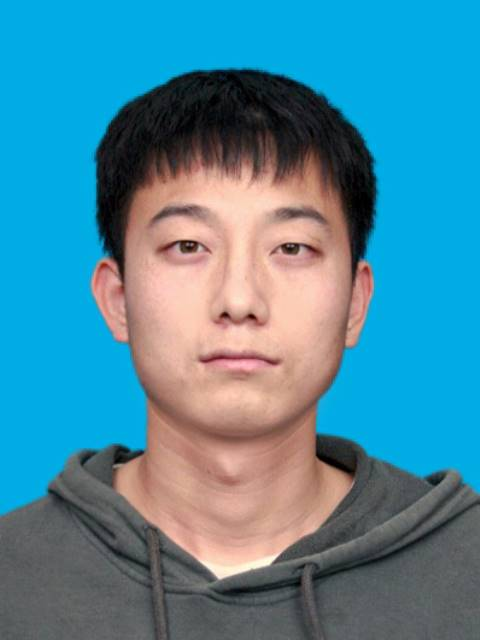
\includegraphics[height=2.7cm]{lyp}};
\end{tikzpicture}%
%%%% 利用tikz来定位学校Logo,这里只在第一页显示,如果需要每页都有,可以考虑在页眉、页脚或者background中加入,不过简历也就一两页,无所谓了
\begin{tikzpicture}[remember picture, overlay] 
  \node[anchor = north west] at ($(current page.north west)+(1.0cm,-0.3cm)$) {
\includegraphics[height=2.5cm]{ustcblue.jpg}};
\end{tikzpicture}%
%%%% 利用tikz来定位页脚栏,电子版简历使用,黑白纸质打印效果可能并不好。这里只在第一页显示,如果需要每页都有,页脚或者background中加入。
\begin{tikzpicture}[remember picture, overlay] 
  \node[anchor = south,fill=CVBlue,draw=none,minimum width=\paperwidth,minimum height=1.5em,align=center,font=\footnotesize,text=white] at ($(current page.south)$) {\faWechat \ passion------lvov(15608482939) \qquad \faGithub \ https://github.com/Masterlvov \qquad \faRssSquare \ http://yp-lv.tk};
\end{tikzpicture}%
%tikzpicture环境很敏感,注释周围的空格、空行都会引起水平距离或垂直距离的变化,
%
\centerline{\LARGE\bfseries{吕永鹏}}

\centerline{\normalsize{应届硕士生,研究方向:金属负极保护 ,求职意向:电芯研发工程师}}

\centerline{\normalsize{\faPhone\ (+86)156-0848-2939 \quad \faEnvelopeO\ \href{yplv@mail.ustc.edu.cn}{yplv@mail.ustc.edu.cn}}}

 
\section{\makebox[\widthof{\faGraduationCap}][c]{\color{CVBlue}\faGraduationCap}\  教育背景}


\textbf{中国科学技术大学} \hfill 2019年9月 -- 2022年6月
%\makebox[\widthof{2020年}][s]{至今}

在读硕士研究生\quad 应用化学与工程学院\quad 专业:化学工程\\
\textit{主修课程}\quad{\quad \quad 电分析化学、能源电化学、电化学研究方法、无机材料表征方法等}

\textbf{中南大学} \hfill 2015年9月 -- 2019年6月
%\makebox[\widthof{2020年}][s]{至今}

本科生(工学学士学位)\quad 化学化工学院\quad 专业:化学工程与工艺\\
\textit{主修课程}\quad{\quad \quad  物理化学、化工原理、化学反应工程、化工热力学、高分子化学等}


\section{\makebox[\widthof{\faGraduationCap}][c]{\color{CVBlue}\faUsers}\ 项目经历}

\textbf{\large{研究生实验室课题}}\  \hfill 2020年4月 -- 2021年4月\\
高比能锂/钠复合空气电池集成及性能提升规律(锂金属负极保护)

\begin{itemize}
  \item 优化锂氧气电池电解液体系,提升了锂氧气电池的循环寿命
  \item 制备钌碳管催化剂以提高锂氧气电池正极反应活性
  \item 对锂负极进行改性保护,极大提升了对称电池以及空气电池的循环时长
  \item 对基本的电化学研究方法进行了一些锻炼
\end{itemize}



\textbf{\large{南京化学工业有限公司和扬子石化有限公司}}\  \hfill \normalsize{2018年7月 -- 2018年8月}\\
生产工艺实习
\begin{itemize}
  \item 在氯碱工业等工厂进行参观学习
  \item 对南化如何空分、制氨等工艺流程实地学习
  \item 对杨子石化生产工艺和自动化控制工艺进行了学习
\end{itemize}



\textbf{\large{湖南省湘潭市燕京啤酒有限公司}}\  \hfill \normalsize{2017年7月 -- 2017年8月}\\
生产工艺实习
\begin{itemize}
  \item 学习了啤酒生产的工艺流程
  \item 学习了啤酒厂厂区布置原理
\end{itemize}

\section{\makebox[\widthof{\faGraduationCap}][c]{\color{CVBlue}\faCogs}\ 技能和兴趣}
% increase linespacing [parsep=0.5ex]
\begin{itemize}[parsep=0.5ex]
  \item 技能:XRD、SEM、TEM等表征手段,熟练使用常用的电化学测试方法(CV、CA、EIS、GITT等)
  %\item 算法:掌握常用的算法与数据结构,熟悉常用的机器学习算法
  \item 英语:通过CET-6,可无障碍阅读英文文档
  \item 办公:能熟练掌握各种办公软件的使用(Office、Origin、排版工具Markdown、\LaTeX 等)
  \item 性格:认真细致、热情活泼、乐于助人、有团队意识
  \item 爱好兴趣:喜欢打篮球,乒乓球,跑步,听歌
  \item 编程语言: MATLAB、\LaTeX、Python 有一些了解
\end{itemize}




\section{\makebox[\widthof{\faGraduationCap}][c]{\color{CVBlue}\faInfo}\ 获奖情况}
% increase linespacing [parsep=0.5ex]
\begin{itemize}[parsep=0.5ex]
  \item \textit{中国科学技术大学研究生一等学业奖学金}\  \hfill{2020 年 9 月}
  \item \textit{中国科学技术大学研究生二等学业奖学金}\  \hfill{2019 年 9 月}
  \item \textit{中南大学化学化工学院芳源杯篮球比赛第四名}\  \hfill{2017 年 6 月}
  \item \textit{中南大学三等校级奖学金}\  \hfill{2017 年 9 月}
\end{itemize}



%%%% 如果多页简历,可以手动在适当位置插入 \newpage 或者 \clearpage 开始新一页

\end{document}
